\documentclass[default]{sn-jnl}
\usepackage{interval}
\usepackage{wasysym}
\usepackage{caption}


% Input, output
\algnewcommand\algorithmicinput{\textbf{Input:}}
\algnewcommand\Input{\item[\algorithmicinput]}
\algnewcommand\algorithmicoutput{\textbf{Output:}}
\algnewcommand\Output{\item[\algorithmicoutput]}


\begin{document}

\title[Tomography Based Technique for Predicting Prognosis in COPD Patients]{A Study on Computed Tomography Based
Technique for Predicting Prognosis in Patients with Chronic Pulmonary Lung Disease (COPD)}

\author*[1]{\fnm{Hao} \sur{Yu}}\email{ethan@dgu.ac.kr}

\author[1]{\fnm{Nnubia Pascal} \sur{Nnamdi}}\email{nubee@dgu.ac.kr}

\author[2]{\fnm{Jinkyeong} \sur{Park}}\email{drjinnie@dgu.ac.kr}

\author[1]{\fnm{Yunsik} \sur{Son}}\email{sonbug@dongguk.edu}

\affil*[1]{\orgdiv{Department of Computer Science and Engineering}, \orgname{Dongguk University},
    \orgaddress{\street{30 Phildong-ro 1gil, Jung-Gu}, \city{Seoul}, \postcode{04620}, \country{Korea}}}

\affil[2]{\orgdiv{Department of Internal Medicine}, \orgname{Dongguk University College of Medicine},
    \orgaddress{\street{32 Dongguk-ro, Ilsandong-gu}, \city{Goyang-si}, \postcode{10326}, \state{Gyeonggi-do},
        \country{Korea}}}

\abstract{Recently, there has been a gradual increase in research on diaphragm functions fused with computer
engineering-related techniques in the medical field. Therefore, this paper proposes a technique for evaluating the
function of the diaphragm through chest computed tomography for chronic obstructive pulmonary disease (COPD)
substitution. The proposed technique utilizes a patient’s chest segmentation algorithm to extract the diaphragm region
from 2D slice images, and calculate the dynamic change experienced during breathing by calculating the diaphragm area
and volume difference during inhalation and exhalation.}

\keywords{Digital image processing, Medical image computing, Computed tomography, Chronic obstructive pulmonary disease,
    Diaphragm segmentation}

\maketitle

\section{Introduction}\label{sec:introduction}

Chronic Obstructive pulmonary disease (COPD) is mainly characterized as progressive irreversible obstruction of airflow
to the lungs and has become a severe health problem in some patients leading to a fatal effect on diaphragm function, In
COPD patients, the diaphragm is the most important muscle in breathing and is closely related to the patient’s dyspnea
symptoms and the mobility of the diaphragm. Despite the fact that the analysis of CT images has been actively used to
diagnose many lungs disease, only a few research has been conducted to evaluate lung function based on the mobility of
the diaphragm.

\section{Related Work}\label{sec:related_work}

COPD is comprised of two main components, which are emphysema and small airway disease. Previous studies show the
results of a quantitative CT assessment significantly correlate with the COPD exacerbation frequency independent of the
severity of airflow limitation. Also, Automated quantitative analysis techniques have been developed to segment the lung
parenchyma and airways from the chest wall and surrounding structures. Furthermore, a high-resolution Computed
Tomography-based approach has also been implemented in diagnosing patients with Fibrosing Interstitial Lung Disease.

\section{Experimental Design}\label{sec:experimental_design}

The figure~\ref{fig:flowchart} explains the process in which 2D images (DICOM Images) of the COPD patients are first analyzed
and converted the JPEG images and thereafter the segmentation of the diaphragm region is conducted. Finally, the
segmented diaphragm region is visualized in 3D image format.

\begin{figure}[htp]
    \centering
    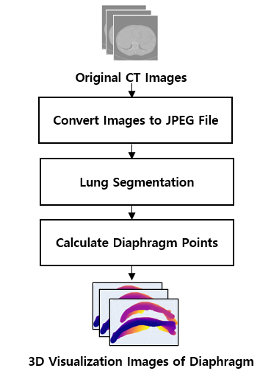
\includegraphics[width=4.4cm]{img/flowchart}
    \caption{Flowchart describing the diaphragm segmentation procedure}
    \captionsetup{justification=centering}
    \label{fig:flowchart}
\end{figure}

\section{Technique Interpretation}\label{sec:technique_interpretation}

\subsection{Background}\label{subsec:background}

As shown in figure~\ref{fig:diaphragm_position}, the position of the diaphragm during inhalation and exhalation is
different, hence the algorithm~\ref{alg:extract_points} is used to obtain continuous diaphragm points during inhalation
or exhalation and merge them for 3D visualization.

\begin{figure}[htp]
    \centering
    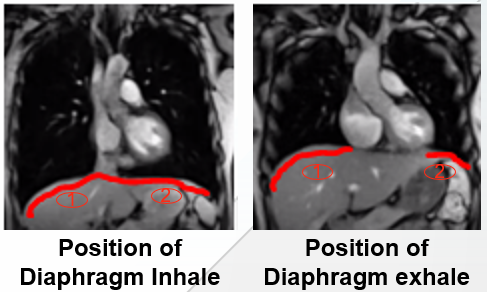
\includegraphics[width=5cm]{img/diaphragm_position}
    \caption{Flowchart describing the diaphragm segmentation procedure}
    \captionsetup{justification=centering}
    \label{fig:diaphragm_position}
\end{figure}

\subsection{Algorithm}\label{Algorithm}

To provide a systematic approach on performing the Computed Tomography Based Technique (CTBT) for predicting prognosis
in patients with COPD the following steps are implemented.

First, Dicom images are viewed through the Dicom viewer known as Horos. Afterward, the Dicom files are converted to JPEG
images. Second, the segmentation of the lungs is conducted first, and then the diaphragm region is segmented using the
OpenCV library. Third, the extreme X and Y axis points are determined. In order to determine the exact diaphragm area,
calculate the second monotonic change point (SMP) from the point with the largest y value to the extreme point of x
(point with the largest x value for the left lung, point with smallest y value for the right lung). If it fails to find
the SMP, the point where the first slope is 0.5 is regarded as SMP. Finally, linearly interpolate the resulting array.

\begin{algorithm}
    \caption{Procedure for extracting diaphragm points from CT images of lungs during inhalation or exhalation}
    \label{algo1}
    \label{alg:extract_points}
    \begin{algorithmic}[1]
        \Ensure{One based indexing for the DCM images}
        \Input{$m, n$ represent the start and end index of the manually selected lung slice image with the diaphragm.}
        \Output{$PTS$ represents the array of linearly interpolated diaphragm points.}
        \Procedure{ExtractPoints}{$DCM_k$, $m$, $n$}
        \State $PTS \Leftarrow \text{new Array}$
        \For {$i = m : n$}
            \State $JPG_i$ \Leftarrow \Call{DCM2JPG}{$DCM_i$}
            \State $HSV_i$ \Leftarrow \Call{BGR2HSV}{$JPG_i$}
            \State $ROI_i$ \Leftarrow \Call{COLOR\_SEG}{$HSV_i$, $lower\_bound$, $upper\_bound$}
            \State $contours_i$ \Leftarrow \Call{CV\_FIND\_CONTOURS}{$ROI_i$}
            \State $x_{extreme}, y_{\max}$ \Leftarrow \Call{GET\_EXTREME\_POINTS}{$contours_i$}
            \State $SMP$ \Leftarrow \Call{2ND\_MONOTONIC}{$x_{extreme}$, $y_{\max}$, $contours_i$}
            \If {$SMP = Null$}
                \State $SMP$ \Leftarrow \Call{ONE\_HALF\_SLOPE\_POINT}{$x_{extreme}$, $y_{\max}$, $contours_i$}
            \EndIf
            \State $TMP_{PTS}$ \Leftarrow $ contours_i$\interval{\Call{ind}{$y_{\max}$}}{\Call{ind}{$x_{extreme}$}}
            \State $TMP_{PTS}$ \Leftarrow \Call{LINEAR\_INTERPOLATION}{$TMP_{PTS}$}
            \State \Call{$PTS$.insert}{$TMP_{PTS}$}
        \EndFor\\
        \hspace{\algorithmicindent}\Return $PTS$
        \EndProcedure
    \end{algorithmic}
\end{algorithm}


\section{Result}\label{sec:result}

Figure~\ref{fig:3d_comparison} compares the 3D results obtained after conducting segmentation of a patient with COPD
(Patient 1) and another patient with acute exacerbations of COPD (Patient 2).

\begin{figure}[htp]
    \centering
    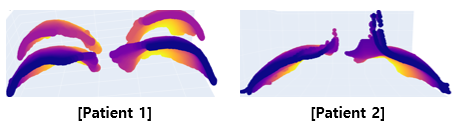
\includegraphics[width=7cm]{img/3d_comparison}
    \caption{Comparison Between patients with COPD}
    \captionsetup{justification=centering}
    \label{fig:3d_comparison}
\end{figure}

Table~\ref{tab:lung_capacity} shows the lung capacity of the two patients. The difference in volume between the two 3D
images indicates a lung capacity difference.

\begin{table}[h]
\begin{center}
\caption{Lung Capacity in both patients}\label{tab:lung_capacity}%
\begin{tabular}{@{}lc@{}}
\toprule
Dataset & Lung Capacity (\%) \\
\midrule
Patient 1 & 72\% \\
Patient 2 & 35\% \\
\botrule
\end{tabular}
\end{center}
\end{table}


\section{Conclusion}\label{sec:conclusion}

In this paper, after further research on the proposed tomography-based technique, it can be actively introduced into
clinical practice through automatic measurement algorithms, this approach has the tendency to aid in respiratory
rehabilitation in patients with chronic obstructive pulmonary disease and can induce the patient’s independent function
recovery thereby increasing the chances of survival.

\backmatter

\bmhead{Acknowledgments}

This research was supported by the MIST (Ministry of Science and ICT), Korea, under the national program for excellence
in SW (No. 2016-0-00017) and the ITRC (Information Technology Research Center) support program
(No. IITP-2021-2020-0-01789) supervised by the IITP (Institute for Information & Communications Technology Promotion).

\bibliography{sn-bibliography}

\input sn-sample-bib.tex

\end{document}
